 \chapter{Introduction}


Code-breaking games (sometimes also called \emph{deductive games} or \emph{searching games})
  are games of two players in which the first player,
  usually referred to as \emph{the codemaker},
    chooses a secret code from a given set, and the second player,
  usually referred to as \emph{the codebreaker},
    strives to reveal the code through a series
    of experiments that give him partial information about the code.

\begin{wrapfigure}{r}{0.32\textwidth}
  \vspace{-5mm}
  \begin{center}
  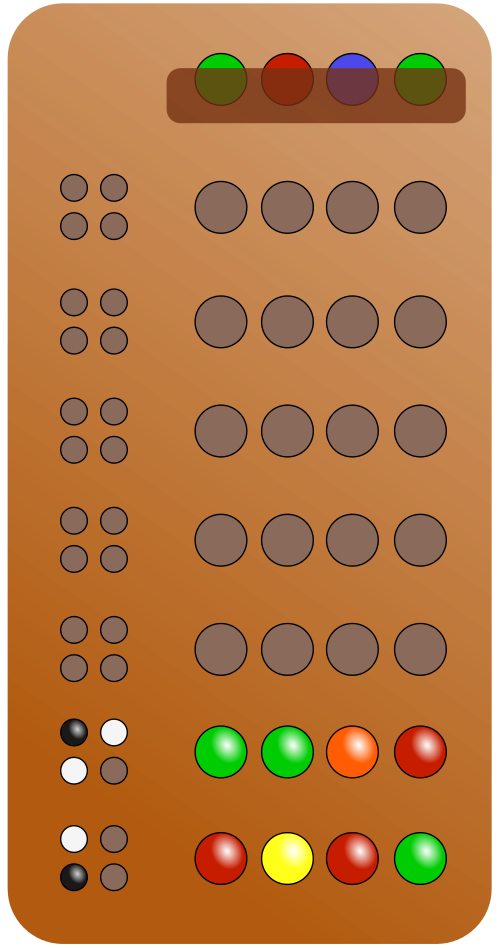
\includegraphics[width=0.25\textwidth]{pictures/mastermind.png}
  \vspace{-5mm}
  \end{center}
  \caption{Mastermind game (illustrative image)\protect\footnotemark.}
  \vspace{-5mm}
\end{wrapfigure}
\footnotetext{Image adopted from \url{http://commons.wikimedia.org/wiki/File:Mastermind\_beispiel.svg}, by Thomas Steiner under GFDL.}

One prominent example of a code-breaking game is famous board game
  \emph{Mastermind}.
In this game, the codemaker creates a puzzle for the codebreaker by choosing a
  combination of four coloured pegs (with colour repetitions allowed).
The codebreaker makes guesses about the colours, which are evaluated by the codemaker with
  black and white markers.
A black marker corresponds to a position where the code and the guess match.
A white marker means that some colour is present both in the code
  and in the guess but at different positions.

Another example of a code-breaking game is the \emph{counterfeit coin problem},
  the problem of identifying an odd-weight coin among
  a collection of genuine coins using only a balance scale.
The codemaker is not a real player here; the balance scale takes his function
  and evaluates the weighings performed by the codebreaker.
Numerous other examples can be found among various board games and logic puzzles;
 we present some of them in the next chapter.

Code-breaking games offer many interesting research problems.

\begin{itemize}
\item \emph{How should the codebreaker play in order to minimize the number of experiments
   needed to undoubtedly determine the code?}
\item \emph{Is there a strategy that would guarantee
   revealing the code in at most $k$ steps?}
\item \emph{What strategy is optimal with respect
   to the average-case number of experiments,
   given that the code is selected
   from the given set with uniform distribution?}
\end{itemize}

Synthesis of an optimal strategy is a computationally intensive task.
In some games, the optimal strategy might have a simple
  structure and can be described easily, such as in
  the counterfeit coin problem (see section \autoref{s:coins} for details).
In general, however, the strategy may have complicated structure and


the only way
  to discover an optimal strategy is by considering all possible experiments
  in a given state and analysing the subproblems.

Therefore, one may prefer a suboptimal strategy or heuristic
  for experiment selection,
  which is easier to compute.
This brings about another kind of questions.
Given a strategy,
  how can we compute the worst-case and the average-case number
  of experiments the strategy needs to reveal the code?

Mastermind and the counterfeit coin problem have been subject to
heavy research and most of these questions are at least partially answered.
The exact results and summary of the research in this area are presented
  in \autoref{ch:games}.
Nevertheless, little has been written about code-breaking games in general.
Some authors have suggested general methods (and applied them in one of the games,
  e.g. \cite{cbg-stgopt, cbg-gen}),
  some have vaguely stated that their approach can be applied
  to other games of the same kind but,
  to the best of our knowledge, no one has tried to
  create a general framework and provide
   results for code-breaking games in general.

This work proposes to bridge the gap and provide
  a general framework for code-breaking games.
We develop a general formalism that uses propositional logic to
  represent the secret code and the partial knowledge.
In short, the secret code is encoded as a valuation of
  a set of propositional variables
  and the codebreaker's goal is to discover the valuation
  using a series of experiments.
Each experiment can result in several outcomes,
  which are given in the form of a prepositional formula.

We study strategies for the games in general, with a focus on
  a special class of \emph{one-step look-ahead} strategies,
  strategy analysis and synthesis of an optimal strategy.
For these problems to be computationally feasible, one needs to exploit
  symmetries of the game and neglect symmetric experiments during the analysis
  or strategy synthesis.
Algorithms for symmetry breaking in Mastermind
  based on graph isomorphism have been suggested in \cite{cbg-nauty}.
We generalize this approach and present
  an algorithm for elimination of symmetric experiments
  in general code-breaking games.

The main contribution of this thesis is the design of a computer language for
  code-breaking game specification
  and the development of a computer program that
  loads a game from a file in the defined format
  and performs various tasks with the game.
We name the tool COBRA, the code-breaking game analyser.
COBRA's currently supported tasks are
\begin{itemize}
\item verifying that a game specification is correct
  and sensible (overview mode),
\item simulating the game either interactively, with input from the user, or
  with decisions by specified strategies (simulation mode),
\item analysing a given strategy for experiment selection --
  computing the worst-case and average-case number of experiments needed (analysis mode),
\item synthesizing the worst-case or average-case optimal strategy (optimal mode).
\end{itemize}
Using this tool, we can easily reproduce some of the known results
  for Mastermind and evaluate the same ideas in other code-breaking games.

The thesis is structured as follows.
Chapter 2 introduces several examples of code-breaking games and
  discusses known results, variants of the games and related research.
The general formalism, definitions and symmetry breaking approach
  are described in Chapter 3.
Chapter 4 is dedicated to our tool, COBRA, with descriptions of its usage and
  abilities.
Experimental results with comparisons of analysed strategies
  are presented in Chapter 5.
Finally, Chapter 6 concludes the work with many suggestions for future work
  and possible extensions of the tool.






